\documentclass{template/openetcs_report}
% Use the option "nocc" if the document is not licensed under Creative Commons
%\documentclass[nocc]{template/openetcs_article}
\usepackage{lipsum,url}
\usepackage{supertabular}
\usepackage{multirow}
\usepackage{color, colortbl}
\usepackage{hyperref}
\usepackage{listings}
\usepackage{makeidx}
\usepackage{amsthm}
\newtheorem{remark}{Remark}
\definecolor{gray}{rgb}{0.8,0.8,0.8}
\usepackage[modulo]{lineno}
\graphicspath{{./template/}{.}{./images/}}
\begin{document}
\frontmatter
\project{openETCS}

\newcommand{\define}[1]{\index{#1}\emph{#1}}

%Please do not change anything above this line
%============================

%user specified macros
%\newenvironment{activity}[2][planned]
	{\begin{tabular}{p{0.25\textwidth}@{\hspace{0.05\textwidth}}p{0.7\textwidth}}
			\multicolumn{2}{p{\textwidth}}{\colorbox{black}{\begin{minipage}{1.1cm}\begin{center}\textsc{\footnotesize \textcolor{white}{#1}}\end{center}\end{minipage}}~~\textbf{#2}}\\
	}
	{\end{tabular}}

\newcommand{\entry}[2]{#1:&#2\\}
\newcommand{\website}[1]{Website:&\url{#1}\\}
\newcommand{\desc}[1]{\multicolumn{2}{p{\textwidth}}{#1}\\}

\newcommand{\VV}{Verification \& Validation\xspace}
\newcommand{\vv}{verification \& validation\xspace}

\newcommand{\tbd}{\colorbox{cyan}{\%\%To Be Defined\%\%}}
\newcommand{\tbc}{\colorbox{cyan}{\%\%To Be Confirmed\%\%}}
\newcommand{\todo}[1]{\colorbox{cyan}{\%\%{#1}\%\%}}
\newcommand{\nthng}[1]{}

% The document metadata is defined below

%assign a report number here
\reportnum{OETCS/WP3/D3.5.1.1}

%define your workpackage here
\wp{Work-Package 3: ``Modeling''}

%set a title here
\title{openETCS System Architecture and Design Specification}

%set a subtitle here
\subtitle{First Iteration: ETCS Kernel Functions}

%set the date of the report here
\date{October 2014}


%document approval
%define the name and affiliation of the people involved in the documents approbation here
\creatorname{Bernd Hekele}
\creatoraffil{DB-Netz}

\techassessorname{Uwe Steinke}
\techassessoraffil{Siemens}

\qualityassessorname{Izaskun de la Torre}
\qualityassessoraffil{SQS}

\approvalname{Klaus-R\"udiger Hase}
\approvalaffil{DB Netz}


%define a list of authors and their affiliation here

\author{Bernd Hekele, Peter Mahlmann, Peyman Farhangi}

\affiliation{DB-Netz AG\\
  V\"olckerstrasse 5\\
  D-80959 M\"unchen, Germany}

\author{Uwe Steinke}

\affiliation{Siemens AG}

\author{Christian Stahl}

\affiliation{TWT-GmbH}

\author{David Mentré}
\affiliation{Mitsubishi Electric R\&D Centre Europe}

% define the coverart
\coverart[width=350pt]{openETCS_EUPL}

%define the type of report
\reporttype{Architecture and Design Specification}


\begin{abstract}
%define an abstract here
This document gives an introduction to the architecture of the first openETCS iteration, the openETCS kernel functions. It has to be read as an add-on to the models in SysML, Scade and to additional reading referenced from the document.
\end{abstract}

%=============================
\maketitle

%Modification history
%if you do not need a modification history table for your document simply comment out the eight lines below
%=============================


\section*{Modification History}
\tablefirsthead{
\hline 
\rowcolor{gray} 
Version & Section & Modification / Description & Author \\\hline}
\begin{supertabular}{| m{1.2cm} | m{1.2cm} | m{6.6cm} | m{4cm} |}
%\begin{supertabular}{| c | c | l | l |}
0.1 & all & Initial document providing the structure & Bernd Hekele \\\hline
0.2 & \ref{sss:provposrep} & initial contribution and some pretty printing & Christian Stahl \\\hline
0.3 & all & collecting feedback and completion on initial sections & Bernd Hekele \\\hline
0.4 & all & changed document style to openETCS report improved pretty printing & Peter Mahlmann \\\hline
0.4.1 & all & adding content & Bernd Hekele \\\hline
\end{supertabular}

% list subsubsections in table of contents
\setcounter{tocdepth}{3}

\tableofcontents
\listoffiguresandtables
\newpage
%=============================

%Uncomment the next line if you need line numbers for tracebility when the document is in review
%\linenumbers
%=============================


% The actual document starts below this line
%=============================
\mainmatter

\chapter{Introduction}


\section{Motivation}
\label{sec:Motivation}

The openETCS work package WP3 aims to provide the architecture and the design of the openETCS OBU software as mainly specified in UNISIG Subset-026 version 3.3.0 \cite{subset-026}. 

The appropriate functionality has been divided into a list of functions of different complexity (see the WP3 function list \cite{functions}).

All these functions are object of the openETCS project and have to be analysed from their requirements and subsequently modelled and implemented. With limited manpower, a reasonable selection and order of these functions is required for the practical work that allows the distribution of the workload, more openETCS participants to join and leads to an executable function providing a limited kernel functionality as soon as possible. 

While the first version of this document focuses on the first iteration of work, i.e.~the limited kernel function, the document is intended to grow in parallel to the growing openETCS software.


\section{Objectives}
\label{sec:Objectives}


The first objective of WP3 software shall be
\begin{quote}
	``Make the train run as soon as possible, with minimum functionality, and in the form of a rapid prototype''.
\end{quote}
Note that this does not contradict the openETCS goal to conform to EN50128. After a phase of prototyping, the openETCS software shall be implemented in compliance to EN50128 for SIL4 systems. The major goals of this document can be summarized as follows:
\begin{itemize}
	\item Identification of the functions required for a minimum OBU kernel.
	\item Give an architecture overview regarding the minimum OBU kernel.
	\item Description of the technical approach, i.e.~the process and methods to be used.
	\item Description of the ``road map'' of the minimum OBU kernel functions and the road map thereafter.
\end{itemize}
Note: This document will be extended according to the progress of WP3. 


\section{History}

%-----------------------------------------------------------------------
\section{Goals of the openETCS Modelling Work}
%-----------------------------------------------------------------------
%\tbc
%by Uwe


\subsection{Functional Scope: The Minimum OBU Kernel Function}
\label{sec:FunctionalScopeTheMinimumOBUKernelFunction}

The objective ``Make the train run with a very minimum functionality'' (see Chapter~\ref{sec:Objectives}) shall be in terms of ETCS OBU translated into 
\begin{itemize}
	\item ``The Train moves on a track equipped with balises and determines its position.''
\end{itemize}
That means, for this very first step, the train shall neither supervise the maximum speed nor activate the brakes. The minimum function set shall be limited to:
\begin{itemize}
	\item Receive, filter and manage balise information received from track (see \url{https://github.com/openETCS/SRS-Analysis/issues/12});
	\item Calculate the actual train position based on balise and odometry information (see \url{https://github.com/openETCS/SRS-Analysis/issues/8});
	\item Calculate the distances between the actual train position to track elements in its front.
\end{itemize}
The activities of the first iteration are collected in the openETCS WP3 backlog for the first iteration \cite{firstIteration}.

A more detailed architectural breakdown of these functions is available as a SysML model \cite{sysml-model}. Diagrams used in the document at hand describing the architecture are taken from the model in \cite{sysml-model}.

The functional design is implemented in the Scade Model \cite{scade-model}. Design documents are taken from this model. Design diagrams used in this document are generated from the model. The design documents produced from the scade model are provided in the design location on Github \cite{designFI}.

In addition, the work on this minimum functionality requires to be supported by
\begin{itemize}
	\item The availability of the ETCS language as specified in Subset UNISIG Subset\_026, chapters 7 and 8;
	\item The abiltiy to link intermediate and final results with the requirements of the ETCS specification (subset\_026, etc.). 
\end{itemize}
These supporting prerequisites are under construction and therefore currently not completely operable. How to deal with these restrictions, will be outlined in Chapter 2.

\section{Glossary and Abbreviations}

\textbf{API} Application Programming Interface\\
\textbf{BTM} Balise Transmission Module\\
\textbf{EVC} European Vital Computer\\
\textbf{LRBG} Last Relevant Balise Group\\
\textbf{SRS} System Requirements Specification\\

%==================================================================

\chapter{The openETCS Architecture of the Initial Kernel Functions}

\section{The openETCS Tool Chain and its Impacts on the Actual Model}

For understanding the modelling process and the modeling guidelines, we refer to \cite{wp3-dow}. 

To summarize the design process, the following rules are in use:
\begin{itemize}
\item Papyrus / SysML is used for modelling the architecture. Functions are visible on this SysML level.
\item No behaviour model is allowed on SysML level.
\item For referencing the requirements, links from the SysML model to the requirements document (in ProR) are being used.
\item Details and especially behaviour is modelled in Scade.
\item All interfaces (see also data-dictionary below) are available on bit-level.
\item In the architecture model in SysML, all interfaces are available on a functional level for interfaces inside and outside the model and for interfaces between dedicated functions. Due to tool constrains the current model does not show all details for all interfaces (see the data dictionary \cite{dataDictionary}).
\end{itemize}

The openETCS tool-chain for doing the modelling work consists of the following components:
\begin{description}
	\item[Papyrus] for modelling the architecture (Kepler version).
	In this phase only the Kepler version of the tool can be used due to incompatibilities of the Kepler and the Luna version on the SysML model. The SysML models are stored at \url{https://github.com/openETCS/modeling/tree/master/model/sysml}.
	\item[ProR] for keeping the requirements (REQIF).
	The subset 26 is converted into a REQIF-format and also stored in the modeling repository on Github. The openETCS toolchain supports the linking of SysML model parts to SRS-Requirements. These results are also part of the architecture.
	\item[Scade] for designing and formalising the functions Scade version 15.2 is used.
	The models are stored at \url{https://github.com/openETCS/modeling/tree/master/model/Scade}.
	With the component Scade System Scade also has a component for designing the architecture.
\end{description}

In principle, the synchronisation mechanism of Scade was planned to be used for synchronising the SysML architecture and the Scade models. The idea is to automatically synchronise the SysML types and blocks with the Scade type definitions and the Scade Operators. Unfortunately, with the current set of tools this idea cannot be realised. Instead, we start developing a new Papyrus plug-in which can be used for generating scade models according to the defined SysML blocks

In addition, faults in the Kepler Papyrus version made it difficult for several members of the team to work on different submodels of the openETCS model. The issue will be solved when changing to the Luna version of Papyrus.

\section{The openETCS Application Software Architecture}


The following diagrams are taken from the SysML model \cite{sysml-model}.

\begin{figure}[h]
\centering
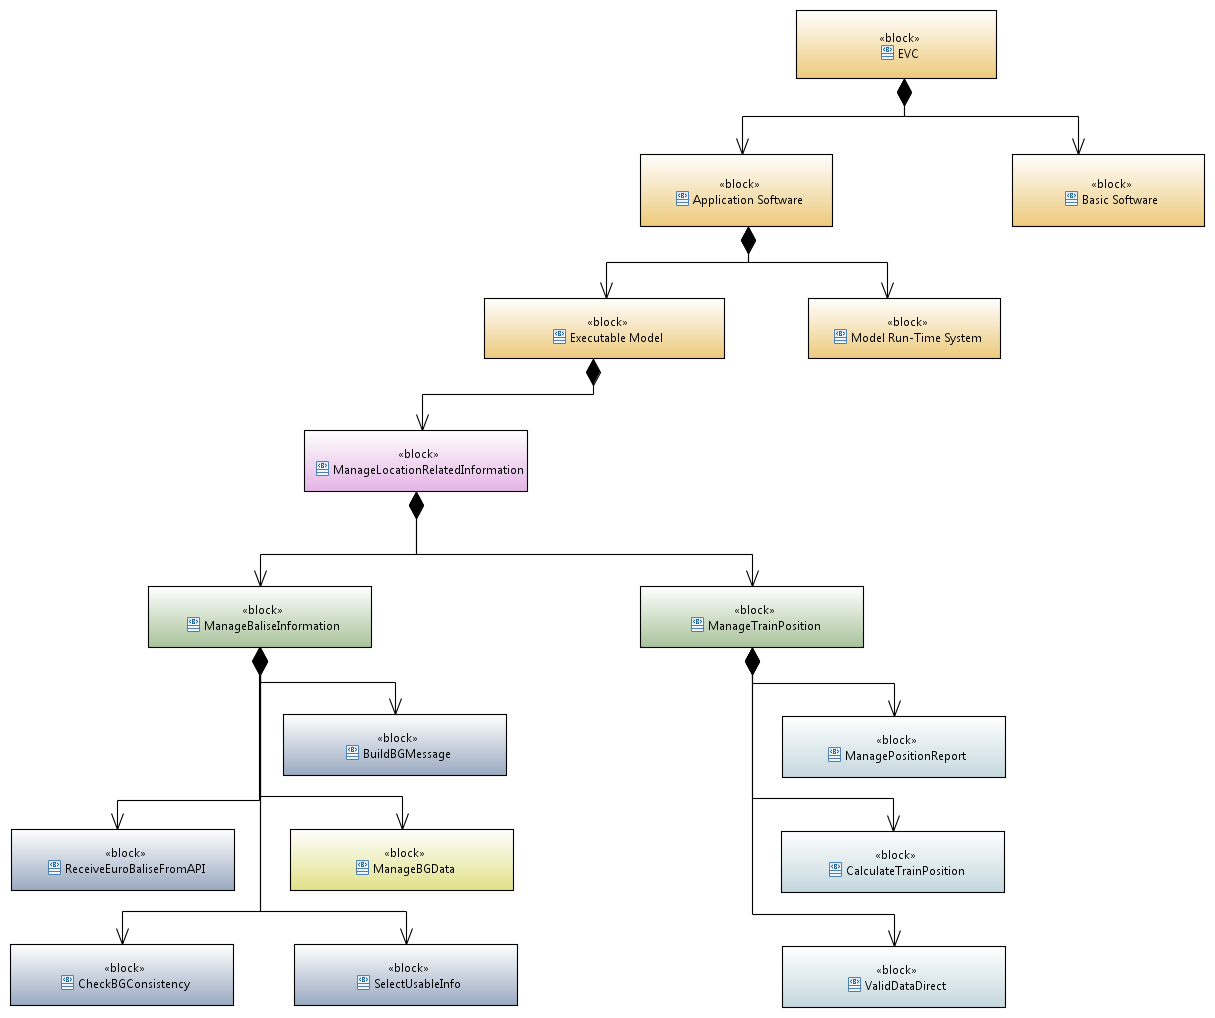
\includegraphics[scale=0.4]{../images/FunctionalArchitectureHigh.png}
\caption{Block Definition Diagram of the First Iteration Architecture}
\end{figure}

The diagram shows the hierarchy of the EVC model. The boundaries of the model are given with the API (interfaces into and outside the EVC model), which actually is not part of the diagram. The runtime system of the EVC is also seen as a part outside the model.

\begin{figure}[p]
\centering
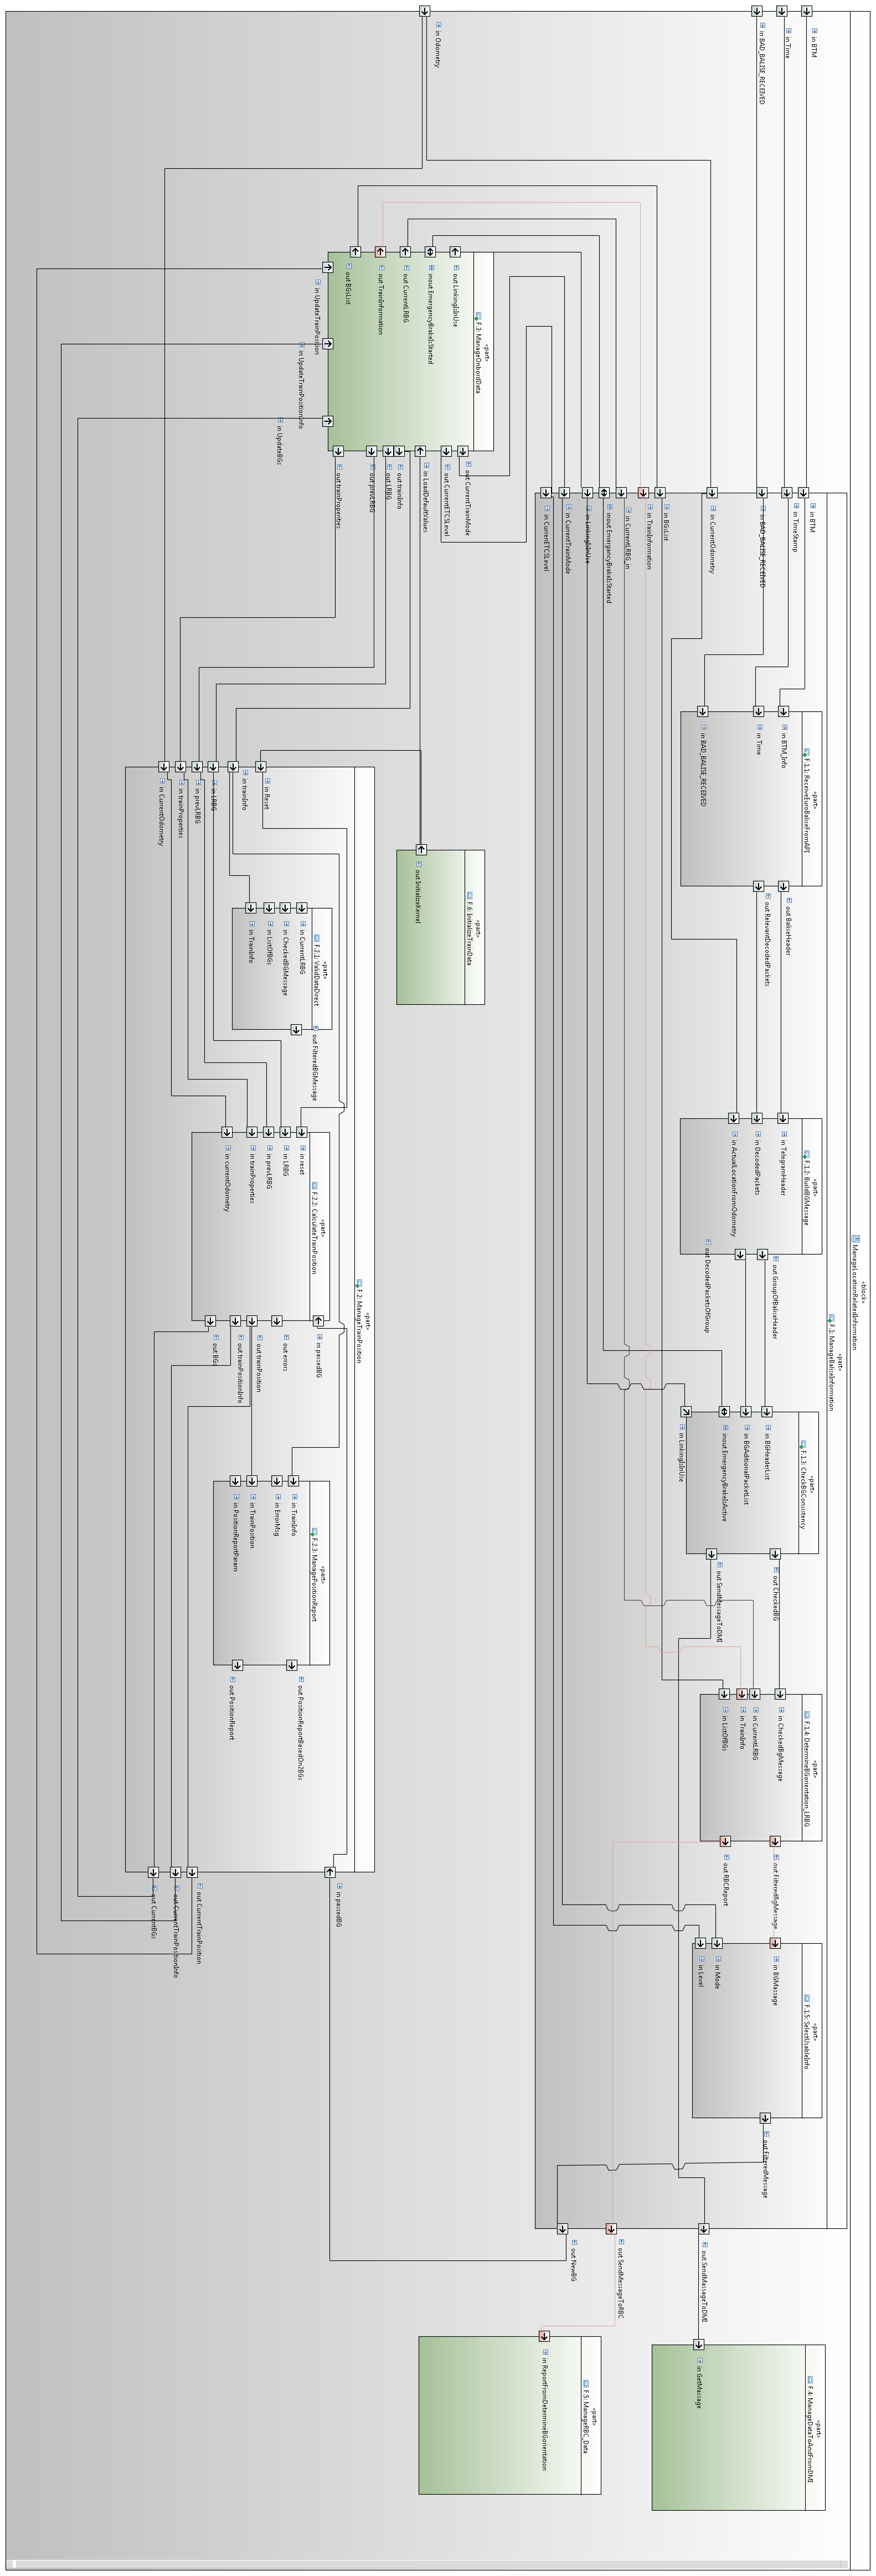
\includegraphics[scale=0.2]{../images/ManageLocationInformationIBD.png}
\caption{Internal Block Diagram of the First Iteration Architecture}
\end{figure}

Green blocks in this diagram are seen as data collected by the ``train'' without making use of the function in focus.

Input to the model is via the Model API (see section 3.1).  

\section{openETCS Data Dictionary}
In the first iteration, the openETCS data dictionary gives some basic constructs for the project, the definition of interfaces in a central place and the definition of the ETCS language \cite{dataDictionary}.

\subsection{ETCS Language}
The type definitions of Subset 26 chapters 7 and 8 (called the ETCS language) are provided as SysML resp. Scade types to the openETCS model. For the SysML model the types have been generated based on tools and provided as <>package<> imported to the openETCS toolschain.



\subsection{openETCS Interfaces}
Interfaces used between submodels and interfaces from outside and to outside the EVC kernel are defined as types in the data dictionary.

In the Scade model the ETCS language is available in the oETCS projects S026-7 and S026-8.

\subsection{Data Dictionary Outlook}
In the first iteration the use of the data dictionary concept is reduced to a minimum. The full openETCS process is tailored for a bigger team to cooperate and make use of tools to collect data and generate code. 

In the Scade model the types needed to build the interface between models are defined in the projects Obu\_Basic\_Types.etp, BG\_Types.etp, and TrainPosition\_Types.etp.


\chapter{openETCS Kernel Functions}

\section{openETCS Model Runtime System}
The openETCS model runtime system also provides:

\begin{itemize}
\item Input Functions from other Units\\\marginpar{maybe use a description}
In this entity messages from other connected units are received.
\item Output Functions to other Units\\
The entity writes messages to other connected units.
\item Conversation Functions for Messages (Bitwalker)\\
The conversion function are triggered by Input and Ouput Functions. The main task is to convert input messages from an bit-packed format into logical ETCS messages (the ETCS language) and Output messages from Logical into a bit-packed format. The logical format of the messages is defined for all used types in the openETCS data dictionary. \\
Variable size elements in the Messages are converted to fixed length arrays with an used elements indicator.\\
Optional elements are indicated with an valid flag.
The conversion routines are responsible for checking the data received is valid. If  faults are detected the information is passed to the openETCS executable model for further reaction. 
\item Model Cycle\\
The executable model is called in cycles. In the cycle 
\begin{itemize}
\item First the received input messages are decoded.
\item The input data is passed to the executable model in a predefined order. \textbf{(Details for the interface to be defined)}.
\item Output is encoded according to the SRS and passed to the  buffers to the units.
\end{itemize}

%==================================================================
\end{itemize}


The openETCS system contains two APIs (Application Programming
Interface):
\begin{enumerate}
\item \emph{openETCS API}: the interface specification between the
EVC platform and the openETCS application;
\item \emph{model API}: the interface between the model itself written in
SCADE and the surounding run-time. Both the SCADE model and the
run-time are making the openETCS application.
\end{enumerate}

\begin{figure}[h]
\centering
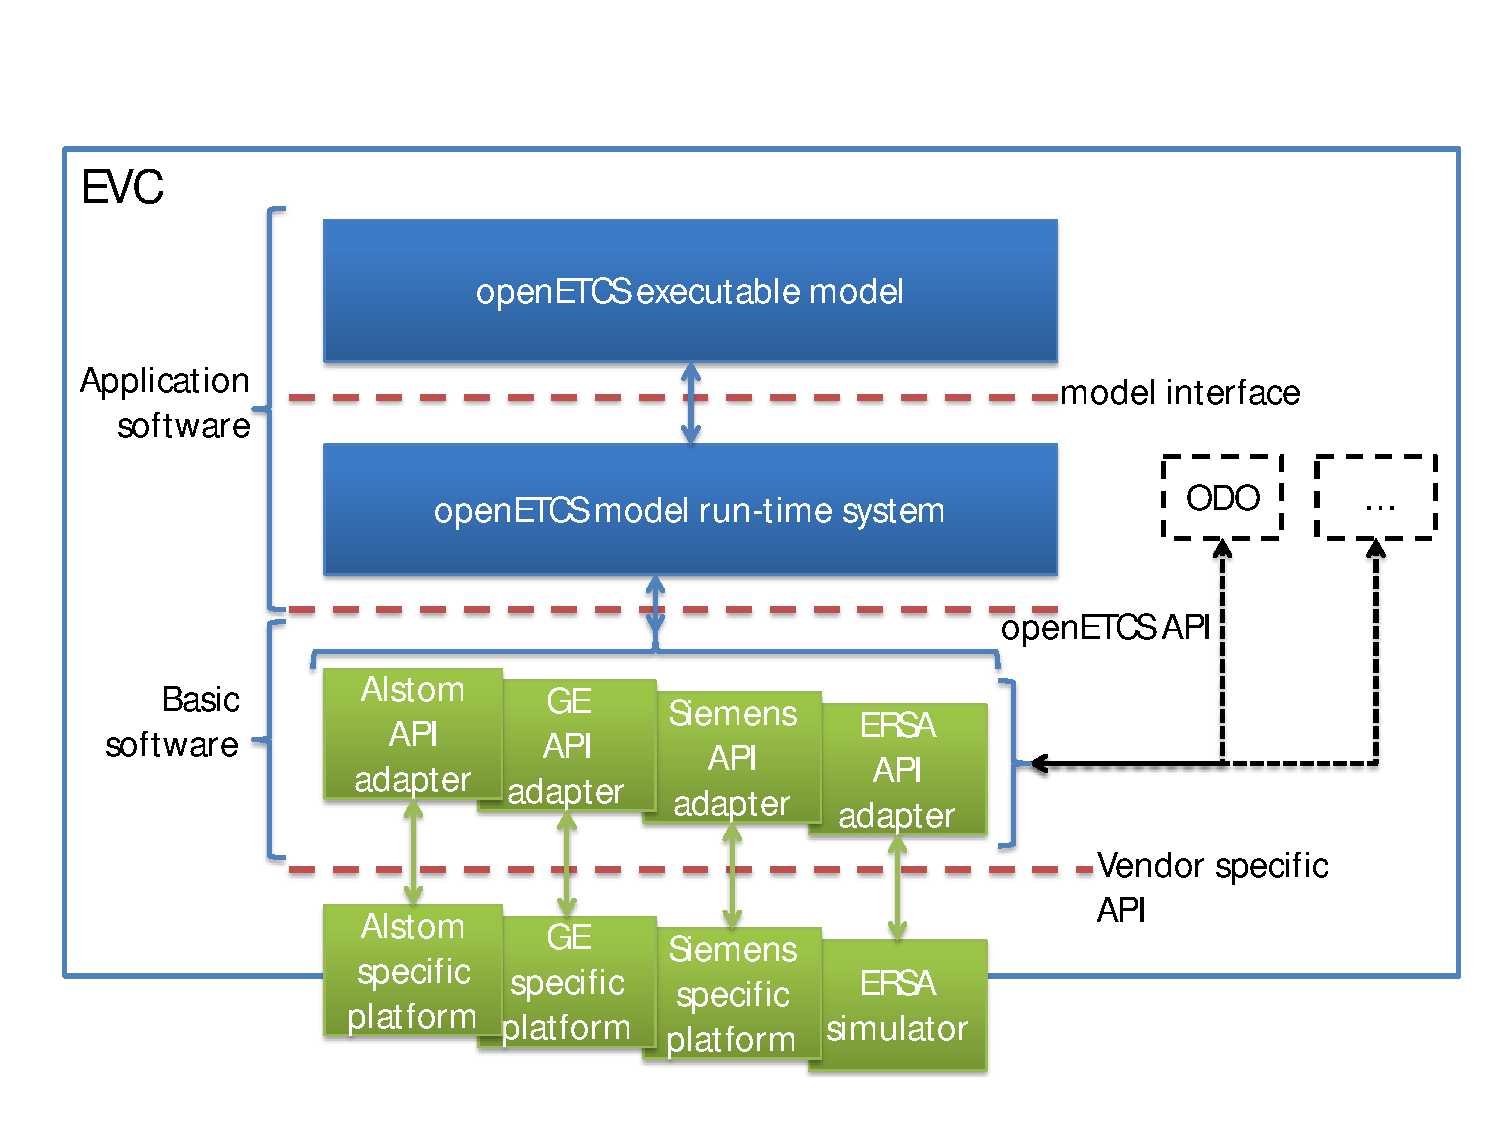
\includegraphics[width=\textwidth]{software-architecture.pdf}
\caption{openETCS software architecture}
\label{fig:software-architecture}
\end{figure}

Figure \ref{fig:software-architecture} shows both openETCS API and
model API on the software stack.

\subsubsection{openETCS API}

The openETCS API is currently defined by two documents, one written by
Alstom \cite{alstom-api} and a more abstract specification written by
openETCS members \cite{openetcs-api}.

The openETCS API defines the interfaces between the EVC platform and
the openETCS application for the following units surrounding the EVC:
\begin{itemize}
\item TIU (Train Interface Unit);
\item ODO (Odometry);
\item DMI (Driver Machine Interface);
\item STM (Specific Transmission Module, up to 8 units);
\item BTM (Balise Transmission Module);
\item LTM (Loop Transmission Module);
\item EURORADIO;
\item JRU (Juridical Recording Unit);
\item Zero or more Vendor specific unit.
\end{itemize}


\subsubsection{Model API}

The model API is currently defined by the inputs and outputs of the SCADE model.

\FIXME{How to give a precise pointer within the SCADE model? Reference
to a specific block within the model?}

For the proper working of the SCADE model, a set of assumptions are assumed:
\begin{itemize}
\item \textbf{Eurobalise (BTM)}: It is assumed that at most one
``telegram'' is provided per call of the SCADE model. This
``telegram'' is the merge of the telegrams of the balises making a
balise group.
\end{itemize}

% LocalWords:  SCADE API openETCS Alstom EVC EURORADIO Odometry balises balise



\section{First Iteration: Model API and Model Runtime System}
Note: The basic functions and the API is not implemented in the first iteration. Instead, the Scade test environment is used for demonstration. However, the interface used in the model is described as if they were available.

\subsection{Short Description of Functionality}

\begin{itemize}
\item Runtime System\\
The Runtime System calls the openETCS kernel model in a cyclic way. Input parameters are updated with every cycle.
\item Input
\begin{itemize}
\item Control Interface\\
The control interface triggers the reset of the application software. The reset is modelled as reset flag in the Scade model.

\item BTM Services\\
The BTM service passes decoded telegrams to the executable model. The telegram is handed over to the API\_balise parameter of the model (see Chapter~\ref{ss:ReceiveEurobaliseFromAPI}). In each cycle only one telegram is expected to be passed.

\item Odometry\\
The input from the odometry is updated with every cycle\marginpar{cycle=clock?}. The information from the odometry is updated in the parameter actual\_odometry of the executable model.
\end{itemize}

\item Output
\begin{itemize}
\item DMI\\
The application may indicate errors at the balise group interface to the driver. The trigger needs to be passed to a corresponding function inside the application software (not part of the kernel).
\item Train Interface Unit (TIU)\\
The application may need the service brake function. The trigger needs to be passed to a corresponding function inside the application software (not part of the kernel).
\item EuroRadio\\
The application may trigger the position report via radio interface. The message needs to be passed to a corresponding function inside the application software (not part of the kernel).
\end{itemize}

\end{itemize}

\section{First Iteration: Interfaces to other Functions of the Application Software (not part of First Iteration)}
This section mainly refers to interfaces replaced by data implemented in the model.

\subsection{Short Description of Functionality}

\begin{description}
\item Train-Info\\
The parameters of the train are seen as a constant to the kernel model. The data re not changed by any function of the kernel model. Only data used in the kernel are listed here.
Used Information: level and mode.
\end{description}

\section{F.1 Manage Balise Information}

\subsection{Short Description of Functionality}

\begin{figure}[hbtp]
\centering
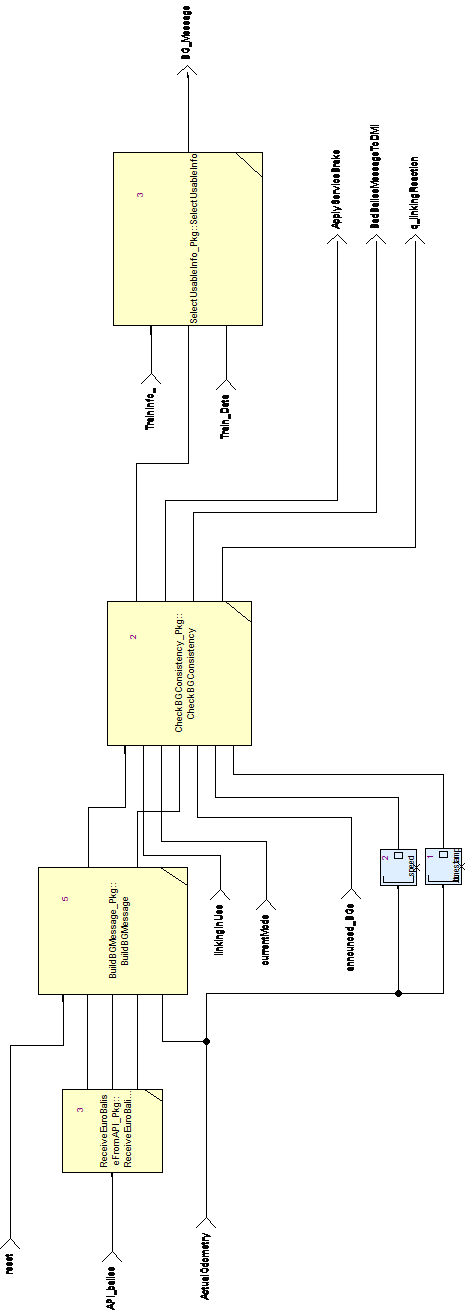
\includegraphics[width=.5\textwidth]{../images/ManageBaliseInformation.png}
\caption{Structure of Manage Balise Information Block}
\end{figure}

"ManageBaliseInformation" manages information related to balise telegrams received via the API when the train passes a balise. Balise telegrams are collected to build balise group messages. Finally, the message is checked for consistency, the train direction is calculated and the balise group message  is passed to the other functions.

Information of the odometer is used to control for the train leaving the expectation window of the balises.

\subsubsection{Input}
\begin{itemize}
\item reset	(bool)	
Request a reset of the data in the function.
If reset=true no other input to the model is valid.
\item API Telegram \\
The telegram is build from 

\begin{itemize}
\item a present flag (bool)\\
Indicates the input decoded telegram parameter is “present”, i.e., the input has been updated by the API.
Only if the telegram is present the position information (incenterOfBalise) is to be used.\\
\item the decoded telegram including optional packets received from the balise.
\item the centerOfBalisePosition parameter. This parameter is used to give the position where the BTM has recognised the center of the balise telegram.
\end{itemize}

\item inActualOdometry\\
Actual Information giving the odometry of the train. 
\item LRBG\\
The Last Relevant Balise Group. The information has been collected before by the train position function.\\
\end{itemize}

\subsubsection{Output}
\begin{itemize}
\item BG-Message\\
Information describing the actual balise group just received.
\item ApplyServiceBreak\\
The flag indicates the balise group the train just passed could not be processed correctly. The check results in the request for a service break.\\
\item BadBaliseMessageToDMI\\
Information to be passed to the DMI to indicate the reception of a "bad balise" to the driver.
\end{itemize}

\subsubsection{Data}
\begin{itemize}
\item The function makes use of internal data for collecting and checking the balise telegrams. 
\end{itemize}

\subsection{Reference to the SRS (or other requirements)}
\begin{itemize}
\item Definition of the Balise Telegram: subset 26 section 7 and 8\\
\item Interface to the BTM: Subset 36, section  4.2.2, 4.2.4, 4.2.9\\
\item Handling of Balise Telegrams: Subset 26, sections 3.4.1 - 3.4.3, 3.16.2 \\
\item Check of the balise group Subset 26, section 3.16.2\\
\item Determining the Orientation: 3.4.2\\
\end{itemize}

\subsection{Design Constraints and Choices}


\subsection{F.1.1 Receive Eurobalise From API}\label{ss:ReceiveEurobaliseFromAPI}

\begin{figure}[hbtp]
\centering
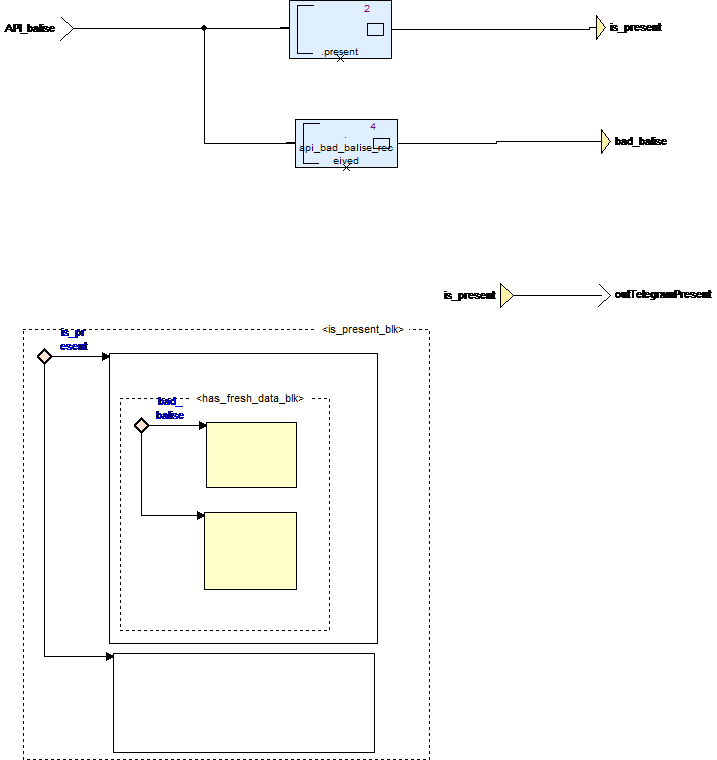
\includegraphics[width=.9\textwidth]{../images/ReceiveEuroBaliseFromAPI_diagram.png}
\caption{Structure of ReceiveEuroBaliseFromAPI}
\end{figure}

\subsubsection{Short Description of Functionality}
This function defines the interface of the OBU model to the openETCS generic API for Eurobalise Messages. On the interface, either a valid telegram is provided or a telegram is indicated which could not be received correct when passing the balise. The function passes the telegram without major changes of the information to the next entity for collecting the balise group information.
	
\subsubsection{Reference to the SRS (or other requirements)}
\begin{itemize}
\item Definition of the Balise Telegram: subset 26 section 7 and 8
\item Interface to the BTM: Subset 36, section  4.2.2, 4.2.4, 4.2.9
\end{itemize}

\subsubsection{Design Constraints and Choices}

\begin{enumerate}
\item The decoding of balises is done at the API. Also, packets received via the interface are already transformed into a usable shape.
\item Only packets used inside the current model are passed via the interface:\\
Packet 5: Linking Information.\\
Linking Information is added to the linking array starting from index 0 without gaps. Used elements are marked as valid. Elements are sorted according to the order given by the telegram sequence.
\end{enumerate}



\subsection{F.1.2 Build BG Group Message}

\begin{figure}[hbtp]
\centering
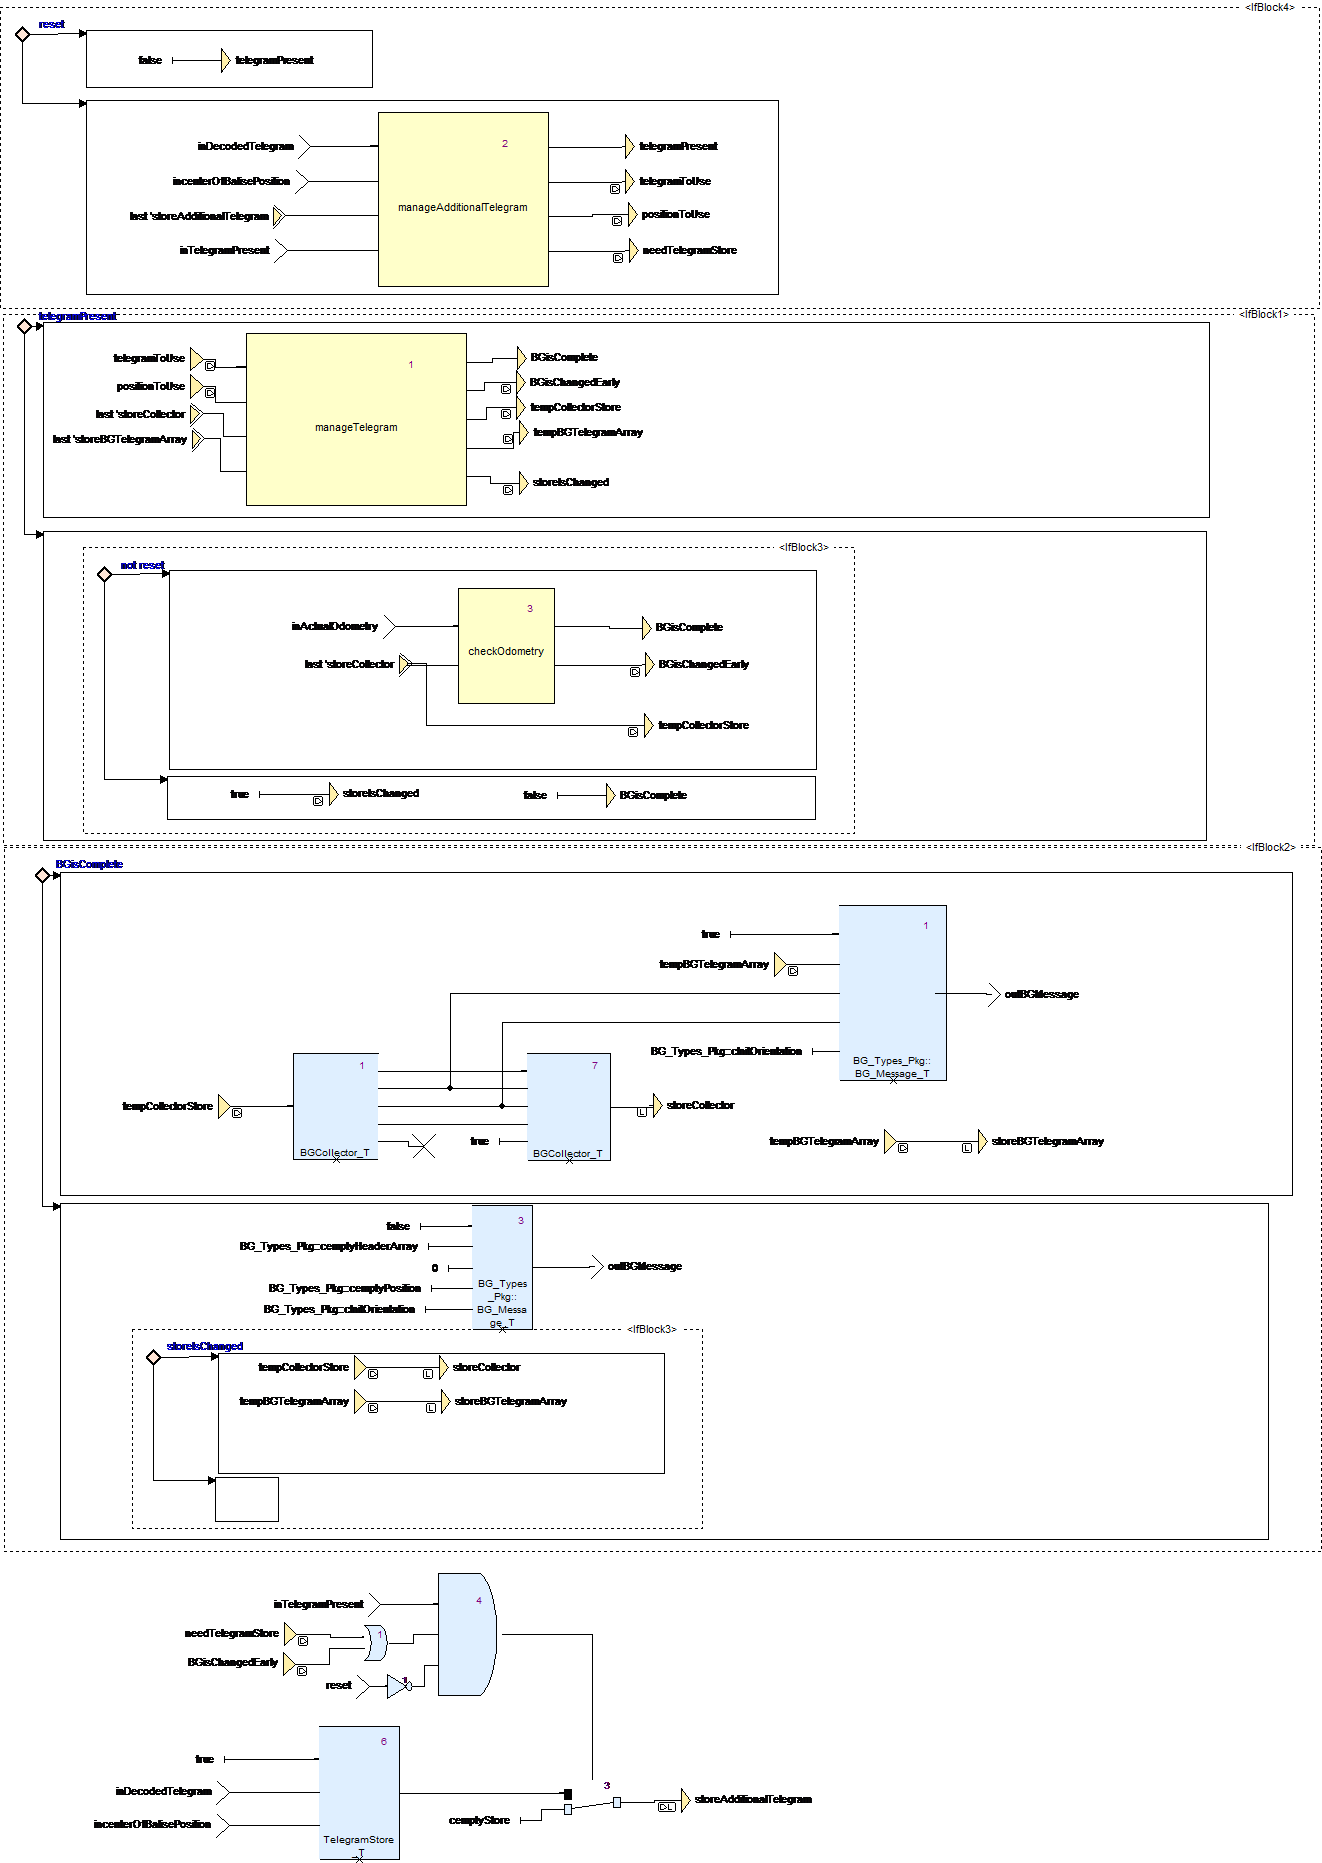
\includegraphics[width=\textwidth]{../images/BuildBGMessage_diagram.png}
\caption{Structure of BuildBGMessage}
\end{figure}

\subsubsection{Short Description of Functionality}
This entity collects telegrams received via the interface into Balise Group Information.
	
\subsubsection{Reference to the SRS (or other requirements)}
\begin{itemize}
\item Interface to the BTM: Subset 36, section  4.2.2, 4.2.4, 4.2.9\\
\item Handling of Balise Telegrams: Subset 26, sections 3.4.1 - 3.4.3, 3.16.2 \\
\end{itemize}

\subsubsection{Design Constraints and Choices}
\begin{enumerate}
\item Telegrams received as invalid are passed to the ``Check-Function'' to process errors in communication with the track side according to the requirements and in a single place.
Telegrams are added to the telegram array starting from index 0 without gaps. Used elements are marked as valid. Elements are stored according to the order given by the telegram sequence.
\item This function does not process information from the packets. The information is passed to the check without further processing of the values. 
\end{enumerate}



\subsection{F.1.3 Check BG Consistency}

\subsubsection{Short Description of Functionality}
This function has the task  to verify the completeness and correctness of the received messages from balis-groups.\\
A message consists of at least a telegram and a maximum of 8 telegrams.\\

\begin{itemize}
\item A message is still complete and correct, if a telegram is missing (or not decoded or incomplete decoded ), and this telegram is duplicated within the balise group and the duplicating one is correctly read.
\item By more than one telegram, the order of the telegrams must be either ascending (nominal ) or Descending(reverse).\\
\item A message is correct, if  all message counters (M MCUNT) do not equal 254 (that means: The telegram never fits any message of the group).\\ A message counter can be equal 255 (that means: The telegram fits with all telegrams of the same balise group) and all other values must be the same.\\
\end{itemize}

\begin{figure}[ht]
\centering
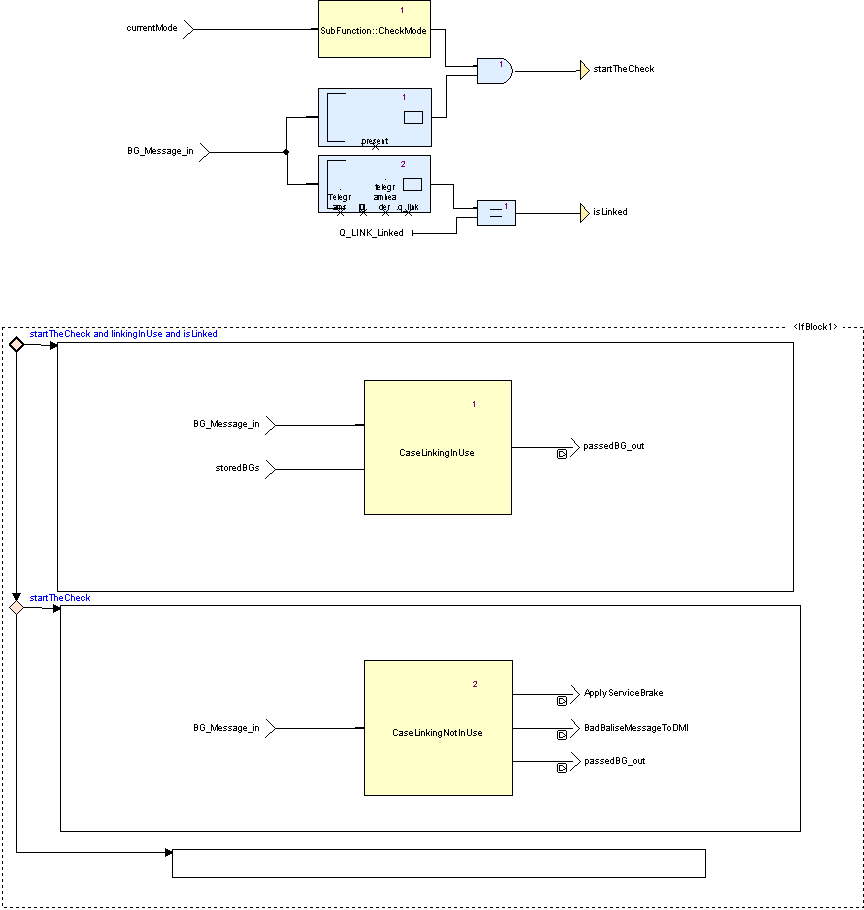
\includegraphics[width=\textwidth]{../images/BGConsistency.png}
\caption{Structure of BGConsistency}
\end{figure}
\subsubsection{Reference to the SRS (or other requirements)}
\begin{itemize}
\item Check of the balise group Subset 26, section 3.16.2\\
\item Determining the Orientation: 3.4.2\\
\item  Active Functions Table: 4.5.2\\

\end{itemize}

\subsubsection{Design Constraints and Choices}

%\begin{enumerate}
%\item Only packets used inside the current model are passed via the interface:\\
%Packet 5: Linking Information.\\
%\item In this function packets past with the telegrams is accumulated into a balise group information.\\
%\item Further assumption on packet 5 (based on SRS subset 26, section 8.4.1.4)\\
%(In this statement the term ``message'' is ambiguous since it can reflect to a telegram or a balise group message)
%Linking Information can only be passed once. This means, if linking information for the balise group is already collected with one of the earlier telegrams, the information will not be accumulated but overwritten.\\
%\end{enumerate}
This function is active in certain modes and the output and reactions are dependent on if the linking information is used.\\
The orientation of the BG will also be calculated in this block.\
The check, if the message has been received in due time and the right at the right expected location, will be performed in "Calculate Train Position".\\
The checks on the validity of the data in the packets and the validity with respect to the direction of motion will be performed in other modules, e.g. "Validate Data Direction" .\\


\subsection{F.1.4 Determine BG- Orientation and LRBG}

The orientation of the Balise Group is already determined in the check procedure. Due to the relocation of functions this block is not used any more.


\subsection{F.1.5 Select Usable Info}
\begin{remark}
This function has to be seen as a separate part of the system, since the filter of this function is not limited to balise messages but also filters radio messages. Thus, the architecture design will be corrected accordingly in the next iteration of the modelling activities.
\end{remark}

\subsubsection{Short Description of Functionality}
The function Select Usable Info filters information received from balises that have been passed, radio messages, and EUROLOOP messages. Filtering is done depending on the mode of the train, the current ETCS level, the type/content of the information, and the transition media of the information. As neither radio messages nor EUROLOOP are part of the first iteration of work, not all functionality of the filter described in the specification is currently implemented.

\subsubsection{Reference to the SRS (or other requirements)}
The functionality of Select Usable Info is described in Chapter 4.8 of subset-026 \cite{subset-026}. The following list gives an overview of the most important sections for each of the blocks in the model.

\begin{description}
\item[First filter] The first filter, i.e.~the filter on the level, is described in \cite[Chapter~4.8.3]{subset-026}.
\item[Second filter] The second filter, i.e.~the filter on the transition media, is described in\cite[Chapter~4.8.3]{subset-026}.
\item[Third filter]
 The third filter, i.e.~the filter on the modes, is described in \cite[Chapter~4.8.4]{subset-026}.
\item[Transition buffers] Details on the handling of the transition buffers used in the first and the second filter are described in \cite[Chapter~4.8.5]{subset-026}.
\end{description}

\subsubsection{Design Constraints and Choices}
The first iteration of the model takes only balise group messages into account. This implies that a large part of the specification of this function described in subset-026 \cite{subset-026} is not relevant for the first iteration. This in particular applies to the second filter, i.e.~filter on the transition media, because radio messages are not part of the model so far. Moreover, the functionality of the first filter, i.e.~filter on the level, is currently  limited because the first iteration of the model implements ETCS level 1 only.

\section{F.2 Manage Train Position}


\subsection{F.2.1 Validate Data Direction}

\begin{figure}[ht]
\centering
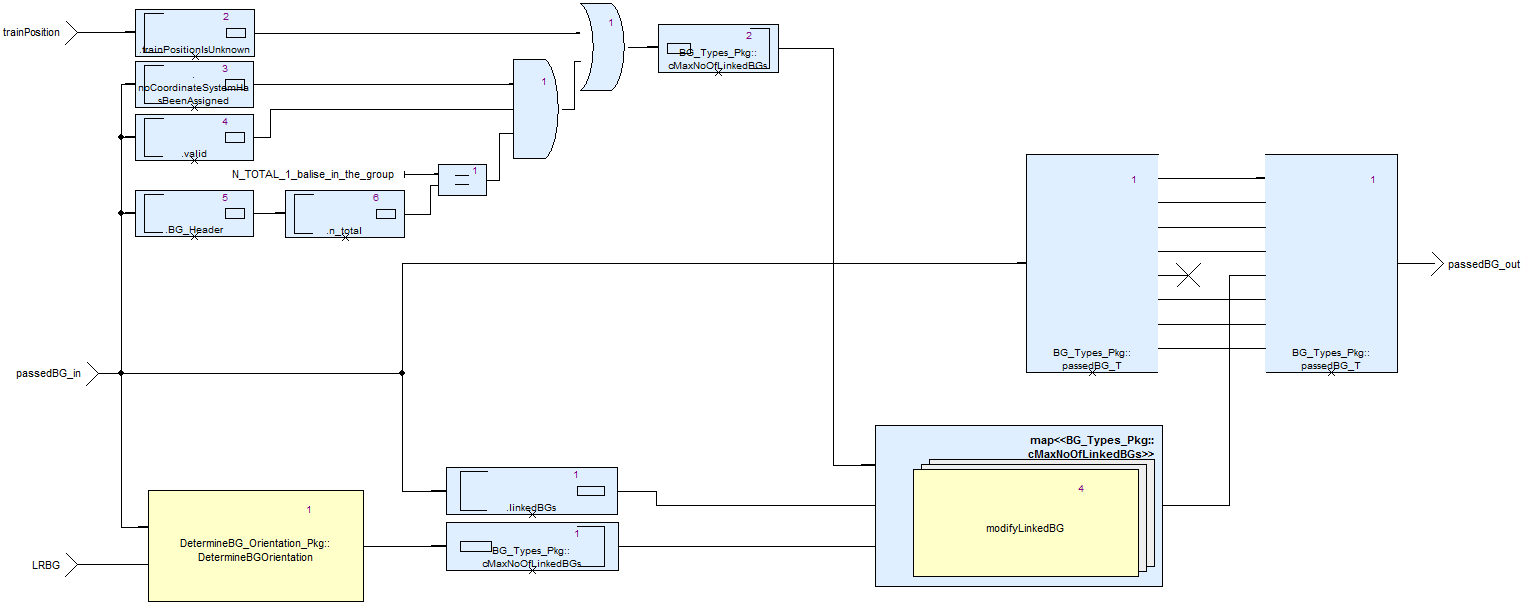
\includegraphics[width=\textwidth]{../images/ValidateDataDirection.pdf}
\caption{Structure of component ValidateDataDirection}\label{fig:validDataDirect}
\end{figure}

\subsubsection{Short Description of Functionality}
This function determines for direction information of the LRBG or an (ordinary) balise group whether this information is valid or not. The function takes as an input the train position, the LRBG and the balise group passed. It outputs the balise group passed extended with validity information. The model consist of two operations and is shown in Figure~\ref{validDataDirect}:
\begin{description}
	\item[DetermineBG\_Orientation] This operation determines the direction in which a BG has been passed.
	%
	\item[modifyLinkedBG] This operation iterates through all LinkedBGs that have announce the BG passed. For each LinkedBG it is checked whether the direction information encoded in \verb+Q_DIR+ is valid w.r.t. the determined BG direction. The special cases described in \cite[Chapter~3.6.3.1.3.1, 3.6.3.1.4]{subset-026} are taken into account using input \verb+singleDirectionInvalid+.
\end{description}

\subsubsection{Reference to the SRS (or other requirements}
The functionality is mainly described in \cite[Chapter~3.6.3]{subset-026}.

\subsubsection{Design Constraints and Choices}
Operation \verb+DetermineBG_Orientation+ is implemented as a package and will be moved to different block in the next iterations. The special case for National Systems as described in \cite[Chapter~3.6.3.1.4.1]{subset-026} has not been modeled yet.

\subsubsection{F.2.2 Calculate Train Position}\label{sss:calctrainpos}

\begin{itemize}
\item \textbf{Short Description of Functionality}\\
The main purpose of the function is to calculate the locations of linked and unlinked balise groups (BGs) and the current train position while the train is running along the track. 

\begin{figure}[hbtp]
\centering
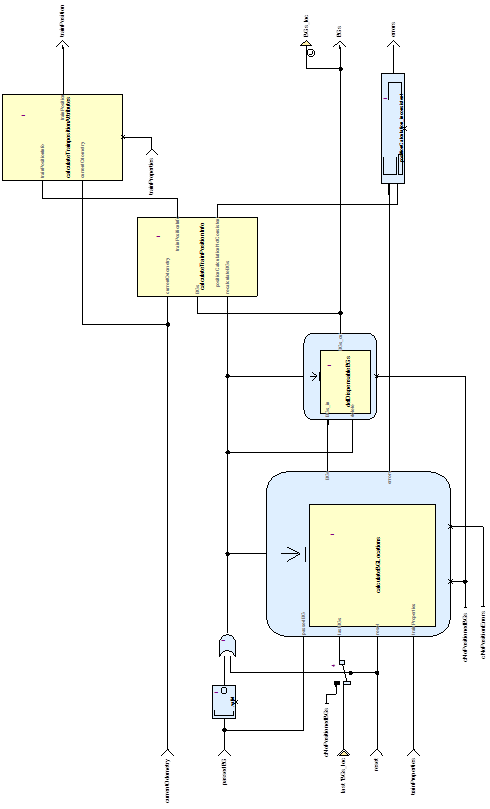
\includegraphics[scale=1]{../images/CalculateTrainPosition.png}
\caption{Structure of calculateTrainPosition}
\end{figure}


\paragraph{Functional Structure in Stages}
The whole function calculateTrainPosition is subdivided into the following steps, which are performed sequentially: 
\begin{enumerate}
\item \textbf{\textit{calculateBGLocations}}: Calculate the balise group locations\\
The first stage is triggered each time the train passes a balise group (input \textit{passedBG}). It takes the balise group header with the BG identification, the linking information (Subset 26, packet 5) and the current odometry values as inputs and calculates the location of the the passed balise group. If the passed BG has been announced via linking information previously, it takes into account the linking as well as the odometry information. If the passed BG does not meet the tolerance window announced by linking, an error flag is set. If the passed BG is an unlinked BG, its location is determined by odometry only, but related to the next previously passed linked BG, if there is one.\\
Then, if the passed BG is a linked BG comprising linking information for BGs ahead, the linking information is evaluated by creating the announced BGs and computing their locations from the linking distances.\\
The passed and the announced BGs are stored in a list \textit{BGs}, ordered by their nominal location on the track.\\
Afterwards the locations of all BGs are further improved by re-adjusting their locations with reference to the just passed BG. This optimizes the BG location inaccuries around the current train position (= location of the passed BG). 

\item \textbf{\textit{delDispensableBGs}}: Delete dispensable balise groups\\
The second stage removes balise groups supposed not to be needed any longer from the list of \textit{BGs}.\\
If the number of stored passed linked BGs exceeds the maximum number of eight as specified in subset-26-3.6.2.2.2 c), all BGs astern are deleted.
If only (passed) unlinked BGs are in the list and exceed the number of \textit{cNoOfAtLeast\_x\_unlinkedBGs}, all passed BGs astern to those are removed from the list. 

\item \textbf{\textit{calculateTrainPositionInfo}}: Calculate train position information.\\
This stage take the list of stored BGs and the current odometry values as inputs and steadily provides the current train position. 

\item \textbf{\textit{calculateTrainpositionAttributes}}: Calculate train position attribute information.\\
This stage provides several additional position related attributes that might conveniently be used by subsequent consumers in the architecture. It requires the actual LRBG and the previous LRBG to be assigned external from the list \textit{BGs}. 

\end{enumerate}

\item \textbf{Reference to the SRS (or other requirements)}\\
\\
The component calculateTrainPosition determines the location of linked and unlinked balise groups and the current train position during the train trip as specified mainly in subset-026-3.6

\item \textbf{Design Constraints and Choices}\\
\\
The following constraints and prerequisites apply:

\begin{enumerate}
\item The input data received from the balises groups must have been checked and filtered for validity, consistency and the appropriate train orientation before delivering them to calculateTrainPosition. 
\item The storage capacity for balise groups is finite. calculateTrainPosition will raise an error flag when a balise group cannot be stored due to capacity limitations.
\item calculateTrainPosition will raise an error flag if a just passed balise group is not found where announced by linking information. It will not (yet) detect when an announced balise group is missing. 
\item calculateTrainPosition is not yet prepared for train movement direction changes. 
\item calculateTrainPosition does not yet consider repositioning information.
\end{enumerate}

\end{itemize}

\subsubsection{Provide Position Report}\label{sss:provposrep}

\begin{figure}[ht]
\centering
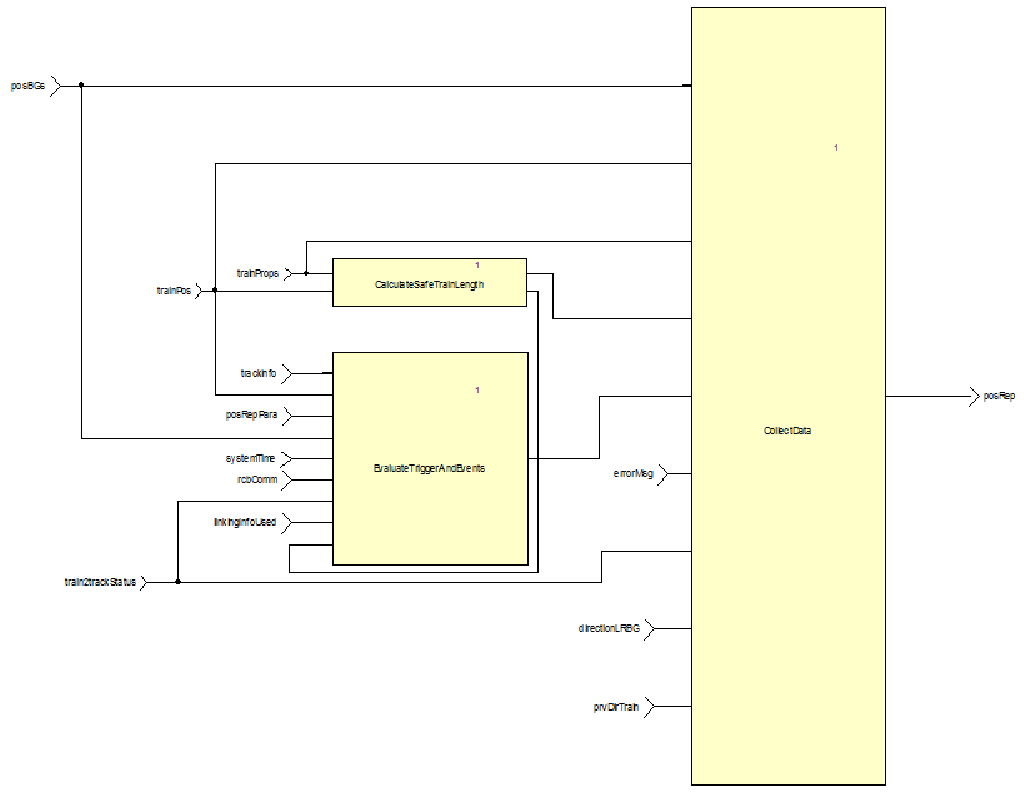
\includegraphics[scale=0.6]{../images/ProvidePositionReport.pdf}
\caption{Structure of component ProvidePositionReport}\label{fig:provideposrep}
\end{figure}

\begin{itemize}
\item \textbf{Short Description of Functionality}\\
This function takes the current train position and generates a position report which is sent to the RBC. The point in time when such a report is sent is determined from event, on the one hand, and position report parameters---which are basically triggers---provided by the RBC or a balise group passed, on the other hand. The functionality is modeled using three operations, as shown in Fig.~\ref{fig:provideposrep}, which are explained below.
\begin{description}
	\item[CalculateSafeTrainLength] Calculates the the safeTrainLength according to Chapt.~3.6.5.2.4/5.
\verb+safeTrainLength = absolute(EstimatedFrontEndPosition - MinSafeRearEnd)+, where
\verb+MinSafeRearEnd = minSafeFrontEndPosition - L_TRAIN+
	\item[EvaluateTriggerAndEvents] Returns a Boolean modeling whether the sending of the next position report is triggered or not. It is the conjunction of the evaluation of all triggers (PositionReportParameters, i.e., Packet 58) and events (see Chapt.~3.6.5.1.4).
	\item[CollectData] In this operation, data of Packet0, \dots, Packet5 and the header is aggregated to a position report.
\end{description}
\item \textbf{Reference to the SRS (or other requirements}\\
Most of the functionality is described in subset 26, chapter~3.6.5.
\item \textbf{Design Constrains and Choices}\\
\begin{enumerate}
	\item The message length (i.e., attribute \verb+L_MESSAGE+) is by default set to 0; the actual value will be set by the Bitwalker/API.
	\item The attribute \verb+Q_SCALE+ is assumed to be constant; that is, all operations using this attribute do not convert between different values of that attribute.
	\item \textit{PositionReportHeader}: The time stamp (i.e., attribute \verb+T_TRAIN+) is not set; this should be done once the message is being sent by the API
	\item \textit{Packet4}: When aggregating the data for this packet, an error message might be overwritten by a succeeding error message. Because the specification only allows to sent one error in one position report, errors are not being stored in a queue, for instance.
	\item \textit{Packet44}: This packet is currently not contained in a position report as it is not part of the kernel functions.
	\item The usage of attributes \verb+D_CYCLOC+ and \verb+T_CYCLOC+ as part of the triggers specified by the position report parameters (i.e., Packet 58 sent by the RBC) may lead to unexpected results if a big clock cycle together with small values for the attributes is used. The cause is that the current model increments at every clock cycle the reference value for the distance and time by at most \verb+D_CYCLOC+ and \verb+T_CYCLOC+, respectively and not a factor of it.
\end{enumerate}
\item \textbf{Open Issues}
\begin{enumerate}
	\item Operation \textit{EvaluateTriggerAndEvents} currently ignores parameters \verb+N_ITER+, \verb+D_LOC+ and \verb+D_LGTLOC+ which allow to specify up to 32 position at which a report has to be sent. The positions are relative to the location of a reference balise group. If the RBC sends packet 58, then it also provides a reference balise group; otherwise, if packet 58 is sent by a balise group, then this balise group serves a the reference balise group. Possible realisation in the model: Extend in the interface posRepPara (i.e., Packet 58) by a \verb+NID_BG+ referring to the reference balise group. Am assumption would be that this BG can be found in the list of passed balise group provided by \textit{CalculateTrainPosition} in Sect.~\ref{sss:calctrainpos}.
	\item The specification requires to store the last eight balise groups for which a position report has been sent (see 3.6.2.2.2.c).
	\item For all reports that contain Packet 1 (i.e., report based on two balise groups), the RBC sends a coordinate system. It is unclear where this has to be stored (i.e., somehow the balise groups have to be stored in a database which has then to be updated), see 3.4.2.3.3.6. Moreover, such a coordination system can be invalid and then has to be rejected (see 3.4.2.3.3.7-8). On a more abstract level, we need to think about the interface between the RBC and the OBU or a proper abstraction thereof.
	\item The decision whether a the report consists of packet 0 or packet 1, which is provided in 3.4.2.3.3, is currently not completely modeled. So far, 3.4.2.3.3.1 has only been modeled, thereby assuming ``the last balise group detected'' is the last balise group and not the LRBG. 3.4.2.3.3.2 is unclear. To model 3.4.2.3.3.4 I need information about the last two valid balise groups and the train running direction. This information can be obtained by adding a memory or this information will be provided by \textit{CalculateTrainPosition} in Sect.~\ref{sss:calctrainpos}. Likewise, also 3.4.2.3.3.5 requires knowledge about the last two valid balise groups.
\end{enumerate}
\end{itemize}


\appendix

%\nocite{*}
\bibliographystyle{unsrt}
%\bibliographystyle{plain}
%\bibliographystyle{alpha}
%\bibliographystyle{annotate}
%\bibliographystyle{klunamed}
\bibliography{architecture}

\newpage
\addcontentsline{toc}{chapter}{Index}
\printindex

%===================================================
%Do NOT change anything below this line

\end{document}
